\documentclass[letterpaper,11pt]{article}
\oddsidemargin -1.0cm \textwidth 17.5cm

\usepackage[utf8]{inputenc}
\usepackage[activeacute,spanish, es-lcroman]{babel}
\decimalpoint
\usepackage{amsfonts,setspace}
\usepackage{amsmath}
\usepackage{amssymb, amsmath, amsthm}
\usepackage{comment}
\usepackage{float}
\usepackage{amssymb}
\usepackage{dsfont}
\usepackage{anysize}
\usepackage{multicol}
\usepackage{enumerate}
\usepackage{graphicx}
\usepackage[left=1.5cm,top=1.5cm,right=1.5cm, bottom=1.7cm]{geometry}
\setlength\headheight{1.5em} 
\usepackage{fancyhdr}
\usepackage{multicol}
\usepackage{hyperref}
\usepackage{wrapfig}
\usepackage{subcaption}
\usepackage{siunitx}
\usepackage{cancel}
\pagestyle{fancy}
\fancyhf{}
\renewcommand{\labelenumi}{\normalsize\bfseries P\arabic{enumi}.}
\renewcommand{\labelenumii}{\normalsize\bfseries (\alph{enumii})}
\renewcommand{\labelenumiii}{\normalsize\bfseries \roman{enumiii})}

\begin{document}

\fancyhead[L]{\itshape{Facultad de Ciencias F\'isicas y Matem\'aticas}}
\fancyhead[R]{\itshape{Universidad de Chile}}

\begin{minipage}{11.5cm}
    \begin{flushleft}
        \hspace*{-0.6cm}\textbf{FI1100 Introducción a la Física Moderna}
    \end{flushleft}
\end{minipage}

\begin{picture}(2,3)
    \put(366, -10){
\includegraphics[scale=0.9]{Imágenes/logo/dfi-fcfm.pdf}}
\end{picture}

\begin{center}
	\LARGE\textbf{Problemitas C3}
\end{center}

\rfoot[]{pág. \thepage}

\section*{\underline{Intro. a la Mecánica Cuántica}}

\begin{enumerate}\setlength{\itemsep}{0.4cm}

\item
\begin{enumerate}
    \item Los fotoelectrones emitidos desde una chapa de cesio iluminada con luz ultravioleta de longitud de onda 2000 {\AA} son detenidos por un potencial de $\SI{4.21}{\V}$. ¿Cuál es la función trabajo del cesio?

    \item La frecuencia media emitida por una bombilla eléctrica de $\SI{200}{\W}$ es $\SI{5.00e14}{\Hz}$, y el $10\%$ de la potencia se emite como luz visible. ¿Cuántos fotones de luz visible se emiten por segundo?
    
    \item Un haz de luz de $\SI{2.50}{\W}$ y con longitud de onda de $\SI{124}{\nm}$ incide sobre una superficie de metal. Usted observa que la energía cinética máxima de los electrones expulsados es de $\SI{4.16}{\eV}$. Suponga que cada fotón en el haz expulsa un fotoelectrón.
    
        \begin{enumerate}
            \item ¿Cuál es la función trabajo de este metal?
            
            \item ¿Cuántos fotoelectrones son expulsados cada segundo de este metal?
            
            \item Si la potencia del haz de luz, pero no su longitud de onda, se redujera a la mitad, ¿cuánto cambia lo obtenido en la parte (b)?
            
            \item Si la longitud de onda del haz, pero no su potencia, se redujera a la mitad, ¿cuánto cambia lo obtenido en la parte (b)?
        \end{enumerate}
\end{enumerate}


\item Vamos a demostrar para un átomo hidrogenoide que $E~\propto~n^{-2}$, para ello:
\begin{enumerate}
    \item Recordando que la fuerza electrostática es de la forma
    $$\left|{\vec{F}}\right| = \frac{K q_1 q_2}{r^2} $$
    
    Utilizando además que $L = n\hbar$, obtenga una expresión para el radio de órbita de un electrón.
    
    \item Recordando que la energía potencial para la fuerza de Coulomb se define como
    $$ U = -\frac{Kq_1q_2}{r}$$
    
    Determine una expresión para la energía.
    
    \item Con esto demuestre que para dos niveles de energía $n, m$ (con $m>n$) se tiene que la transición de un estado de mayor energía a uno de menor energía cumple:
    $$\frac{1}{\lambda} = Z^2 R_H\left(\frac{1}{n^2}-\frac{1}{m^2}\right)$$
\end{enumerate}
\item
    \begin{enumerate}
        \item ¿Cuál es la cantidad mínima de energía que se debe transmitir a un átomo de hidrógeno que al principio está en su nivel fundamental, para que pueda emitir la línea $H_{\alpha}$ de la serie de Balmer?
        
        \item ¿Cuántas posibilidades distintas de emisiones de líneas espectrales hay para este átomo cuando el electrón comienza en el nivel $n = 3$ y termina en el nivel fundamental? Calcule la longitud de onda del fotón emitido en cada caso.
    \end{enumerate}

\item Considere un átomo de berilio (Z=4) al cual se le quitan tres electrones. Para este átomo:
\begin{enumerate}
    \item ¿Cuál es la energía fundamental? Compare con el átomo de Hidrógeno.
    \item ¿Cuál es la energía de ionización? Compare con el átomo de Hidrógeno.
    \item Para el Hidrógeno se tiene que la longitud de onda emitida por un fotón debido a una transición de $n=2$ a $n=1$ es $\SI{122}{\nm}$. ¿Cuál será la longitud de onda emitida de un fotón debido a esta misma transición?
    
    \item Para un valor dado de $n$, compare el radio de órbita de un electrón en este átomo con el hidrógeno.
\end{enumerate}

\item Considere un nuevo modelo de átomo el cual utiliza la Ley de Hooke $\vec{F} = -kr$ como interacción entre protón y electrón. Usando los postulados de cuantización de Bohr y utilizando órbitas circulares

\begin{enumerate}
    \item Calcule los radios de órbita permitidos

    \item ¿Cuáles son las correspondientes velocidades?

    \item ¿Cuáles son las correspondientes energías?

    \item Determine una expresión análoga a la fórmula de Rydberg
\end{enumerate}
\end{enumerate}


\section*{\underline{Óptica Ondulatoria}}

\begin{enumerate}\setlength{\itemsep}{0.4cm}
\item Una cuña de aire se forma entre dos placas de vidrio separadas
por un alambre muy fino. Cuando la cuña es iluminada desde arriba por una luz de $\SI{600}{\nm}$ y se observa desde arriba, aparecen 30 franjas oscuras. Calcule el radio del alambre

\begin{figure}[H]
    \centering
    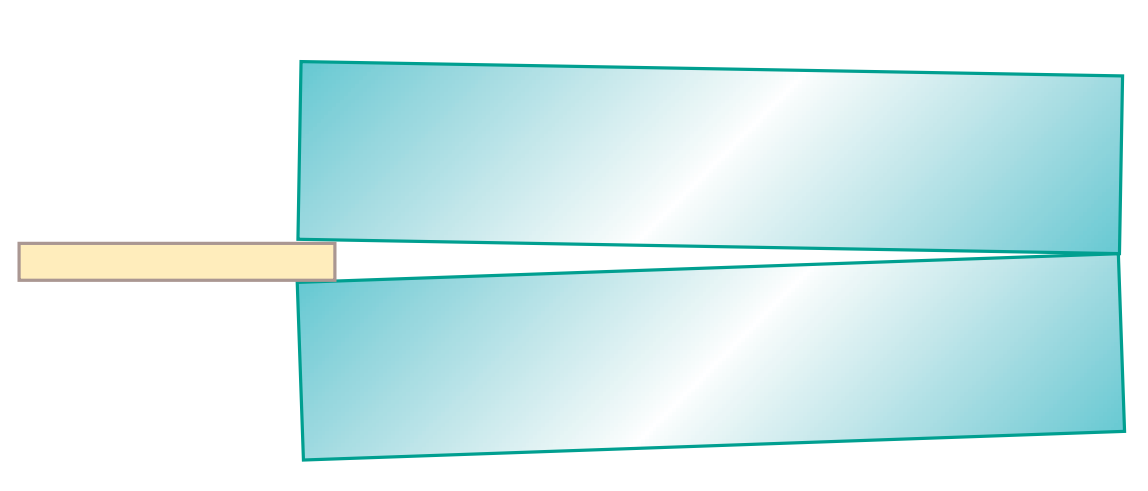
\includegraphics[width=0.3\linewidth]{Imágenes/clases/placas2.png}
\end{figure}

\item \textbf{[P2-C3 2020-2]} Se realiza un experimento de doble rendija usando un láser de He-Ne ($\lambda = \SI{633}{\nm}$). Luego, se coloca un placa muy delgada de vidrio ($n = 1.5$) sobre una de las ranuras. Se observa que el punto central en la pantalla está ahora ocupado por la que había sido la franja oscura correspondiente a $m = 10$. ¿Cuán grueso es el vidrio?
Considere que la pantalla está ubicada muy lejos, de manera que vale la aproximación paraxial (todos los ángulos son muy pequeños).


\item Se hace pasar un láser con longitud de onda 630 nm a través de una ranura angosta y se observa un patrón de difracción en una pantalla a 8 m de distancia. Se encuentra que, en la pantalla, la distancia entre los centros de los primeros mínimos fuera de la franja brillante central es de 32 mm. ¿Cuál es el ancho de la ranura?
\end{enumerate}

\section*{\underline{Sonido}}

\begin{enumerate}\setlength{\itemsep}{0.4cm}

\item Un buque en reposo sobre aguas profundas está equipado con un sonar que envía pulsos de sonido de $\SI{20}{\MHz}$. Los pulsos reflejados en la superficie de un submarino ubicado directamente debajo del barco se demoran $\SI{0.06}{\s}$ en regresar al barco y tienen una frecuencia de $\SI{19.979}{\MHz}$. Considere que la velocidad del sonido en el agua de mar es $\SI{1.48}{\km/\s}$

\begin{enumerate}
    \item Encuentre la profundidad del submarino

    \item Encuentre la velocidad vertical del submarino
\end{enumerate}
\end{enumerate}
\end{document}